% Provenance (never printed): see sources/outline_sources.md (Year 3:
% stereographic projection; fold and fault analysis; palaeostress; balanced
% cross-sections). Brief: sources/book5/BRIEFS.md, ch. 8. Nets, pi-diagram and
% fault-slip data from figdata/bachelor-3/stereonet.py (Varden data invented,
% from figdata/shared/region.py); Fry plot from figdata/bachelor-3/fry.py.
% Exercise and problem values in the Book 5 scratch calculator calc/ch08.py.
% No real-world numbers: no ledger rows.
\chapter{संरचनात्मक विश्लेषण}\label{ch:b3:structural-analysis}

एक भूवैज्ञानिक ने एक वलन के पार्श्वों पर दो सौ संस्तर-तल मापे हैं। यह वलन
इतना बड़ा है कि पूरा देखा नहीं जा सकता: उसका वलन-मोड़ एक जंगल के नीचे है, और
उसके पार्श्व किलोमीटरों तक फैले हैं। प्रत्येक पाठन संख्याओं का एक युग्म है। इन्हें एक वृत्ताकार चार्ट पर बिंदुओं के रूप में आलेखित करने पर
संस्तर-तलों के \omterm{def:b3:structural-analysis:stereo}{ध्रुव} एक ही वक्र के अनुदिश पड़ते हैं, जो एक वृहत् वृत्त है, और
उस वृहत् वृत्त का \omterm{def:b3:structural-analysis:stereo}{ध्रुव} वलन-अक्ष है, वह रेखा जिसे आज तक किसी ने नहीं देखा।
यह अध्याय चार्ट बनाता है, अर्थात \omterm{def:b3:structural-analysis:stereo}{त्रिविम प्रक्षेपण}, और
उसके पीछे के सदिश उपकरणों के साथ उसका उपयोग करता है, ताकि वलन-अक्ष ज्ञात हों, विरूपित वस्तुओं में दर्ज विकृति मापी जा सके,
एक समुच्चय के भ्रंशों को चलाने वाला प्रतिबल पुनः प्राप्त किया जा सके, और
एक विरूपित अनुप्रस्थ काट को विरूपण से पहले की अवस्था में
पुनर्स्थापित किया जा सके।

\begin{recall}
गोले के वृहत् वृत्त और लघु वृत्त पुस्तक 3 (स्नातक वर्ष 1) में हैं, उसके
गोलीय खगोल विज्ञान वाले अध्याय में; स्ट्राइक, नति, नति-दिशा, दिगंश और नमन उसके
भूवैज्ञानिक मानचित्रों और अनुप्रस्थ काट वाले अध्यायों में हैं; नति-दिशा $\alpha$ और नति $\delta$ वाले तल का ऊर्ध्वमुखी एकक अभिलंब,
$\vec n = (\sin\delta
\sin\alpha, \sin\delta\cos\alpha, \cos\delta)$ पूर्वी, उत्तरी और ऊपर के घटकों में, और
पाठनों के एक समुच्चय का सदिश माध्य, जो
क्षेत्र और प्रयोगशाला विधियों पर उसके पहले अध्याय में है। वलन के अवयव और वर्ग,
वलन की मोड़-रेखा, जो $\vec n_1\times\vec n_2$ के समांतर है, और अंतर-पार्श्व कोण
$\ang{180} - \arccos(\vec n_1\cdot\vec n_2)$, तथा एंडरसन का भ्रंशन-सिद्धांत, उसके
भ्रंश, वलन और विन्यास वाले अध्याय में हैं; प्रतिबल,
मुख्य प्रतिबल, विकृति-दीर्घवृत्त और सरल कर्तन उसके
प्रतिबल, विकृति और प्रवाहिकी वाले अध्याय में; सरकन-सदिश का रेक (स्ट्राइक से,
\ang{-90} सामान्य भ्रंश के लिए, \ang{90} उत्क्रम भ्रंश के लिए, 0 बाएँ-पार्श्वीय और
\ang{180} दाएँ-पार्श्वीय), और उद्गम-यांत्रिकी के P और T अक्ष उसके
भूकंप-स्रोत वाले अध्याय में हैं; संतुलित अनुप्रस्थ काट और डेकोलमां
पुस्तक 4 (स्नातक वर्ष 2) में, उसके आल्प्स वाले अध्याय में हैं। न्यूनतम वर्ग
\cref{sec:b3:seismology-imaging:inverse} में हैं; सममित आव्यूह के आइगेनमान और
आइगेनसदिश गणित की पुस्तकों में हैं।
\end{recall}

\section{त्रिविम प्रक्षेपण}\label{sec:b3:structural-analysis:stereo}

एक भूवैज्ञानिक के आँकड़े अभिविन्यास होते हैं: किसी संस्तर-तल का, किसी
भ्रंश का, किसी पर्णन का; और किसी रेखन, वलन-मोड़ या सरकन-दिशा का
दिगंश और नमन। प्रत्येक एक बिंदु से गुजरने वाली दिशा होती है, जिसकी कोई स्थिति नहीं होती। सैकड़ों की तुलना के लिए
मान लीजिए वे सब एक ही गोले के केंद्र तक ला दी गई हैं:
एक रेखा गोले के निचले अर्धगोले को एक बिंदु पर काटती है, और एक तल उसे
एक अर्ध-वृहत् वृत्त के साथ काटता है। निचले अर्धगोले का चार्ट तब रेखाओं को
बिंदुओं और तलों को वक्रों के रूप में दिखाता है।

\begin{definition}[त्रिविम प्रक्षेपण, सम-कोणीय जाल, सम-क्षेत्रफल प्रक्षेपण, ध्रुव]\label{def:b3:structural-analysis:stereo}
मान लीजिए $O$ केंद्र और $R$ त्रिज्या वाला एक गोला है, और उसके केंद्र से होकर जाने वाली एक रेखा निचले
अर्धगोले को $P$ पर काटती है, नादिर से $\theta = \ang{90} - p$ कोण पर, जहाँ
$p$ रेखा का नमन और $t$ उसका दिगंश है। \emph{त्रिविम प्रक्षेपण}\index{त्रिविम प्रक्षेपण} $P$ को उस बिंदु पर भेजता है
जहाँ खमध्य से $P$ तक की सीधी रेखा
क्षैतिज तल को काटती है, जो $O$ से होकर
जाता है: वह बिंदु $r$ दूरी पर, $O$ के सापेक्ष दिगंश $t$ में स्थित होता है। इस प्रकार
बनाया गया निचले अर्धगोले का चार्ट, जिसमें वृहत् और
लघु वृत्तों का जाल है, वह \emph{सम-कोणीय जाल}\index{सम-कोणीय जाल} (या
वुल्फ़ जाल)। \emph{सम-क्षेत्रफल प्रक्षेपण}\index{सम-क्षेत्रफल प्रक्षेपण}
$P$ को उस बिंदु पर भेजता है जिसकी दूरी $r =
R\sqrt2\sin(\theta/2)$ पर और दिगंश $t$ में है। उसका जाल श्मिट जाल कहलाता है।
किसी तल का \emph{ध्रुव}\index{ध्रुव} उसकी अभिलंब रेखा होती है, जिसे
एक बिंदु के रूप में आलेखित किया जाता है: नति-दिशा $\alpha$ और नति $\delta$ वाले तल के लिए,
ध्रुव का दिगंश $\alpha + \ang{180}$ और नमन $\ang{90} - \delta$ होता है।
\end{definition}

दोनों प्रक्षेपण ऊर्ध्वाधर रेखा को केंद्र पर और क्षैतिज रेखा को
त्रिज्या $R$ के वृत्त पर, जो आदिम वृत्त है। वे इस बात में भिन्न हैं कि क्या बनाए रखते हैं।

\begin{theorem}[दोनों प्रक्षेपण]\label{thm:b3:structural-analysis:projections}
\begin{enumerate}[label=(\alph*)]
  \item \omterm{def:b3:structural-analysis:stereo}{त्रिविम प्रक्षेपण} $P$ को $r = R\tan(\theta/2)$ पर रखता है। यह
        कोण-संरक्षी है: प्रत्येक बिंदु पर यह सभी दिशाओं को एक ही गुणक
        $1/(2\cos^2(\theta/2))$ से फैलाता है, ताकि वक्रों के बीच के
        कोण बने रहें।
  \item \omterm{def:b3:structural-analysis:stereo}{सम-क्षेत्रफल प्रक्षेपण} हर क्षेत्रफल को एक ही गुणक से गुणित करता है,
        $1/2$: जाल के किसी क्षेत्र का क्षेत्रफल उस गोलार्ध के क्षेत्र का आधा होता है,
        जिसे वह निरूपित करता है।
\end{enumerate}
\end{theorem}

\begin{proof}
(क) खमध्य $Z$, नादिर और $P$ से होकर जाने वाले ऊर्ध्वाधर तल में
(नीचे का पहला चित्र), नादिर से $P$ तक का चाप
केंद्र पर कोण $\theta$ अंतरित करता है, अतः अंतर्लिखित कोण
$\theta/2$ का अंतर्लिखित कोण $Z$ पर बनता है, जो $R$ दूरी पर $O$ के ऊपर है: $r =
R\tan(\theta/2)$। नादिर की ओर गोले पर एक लघु पद $R\,\mathrm d\theta$
चार्ट पर $\mathrm dr = R\,\mathrm d\theta/(2\cos^2(\theta/2))$ बन जाता है।
नादिर से कोण $\theta$ पर स्थित बिंदुओं का वृत्त, जिसकी परिधि $2\pi R\sin\theta$ है,
चार्ट पर परिधि $2\pi
r$ वाला वृत्त बन जाता है; अनुपात $\tan(\theta/2)/\sin\theta = 1/(2\cos^2(\theta/2))$ है,
जो त्रिज्या के अनुदिश का भी वही है। ऐसा मानचित्र जो दो लंबवत दिशाओं में
समान रूप से फैलाता है, वह सभी दिशाओं में समान रूप से फैलाता है और कोण बनाए रखता है।

(ख) नादिर से कोण $\theta$ के भीतर गोले की टोपी का क्षेत्रफल
$2\pi R^2(1 - \cos\theta) = 4\pi R^2\sin^2(\theta/2)$ है; उसका प्रतिचित्र
क्षेत्रफल $\pi r^2 = 2\pi R^2\sin^2(\theta/2)$ वाली चकती है, यानी उसका आधा। दोनों क्षेत्रफल
दिगंश में समान रूप से बँटे हैं, इसलिए दो दिगंशों के बीच की टोपी का खंड
और उसका प्रतिचित्र अनुपात $1/2$ रखते हैं, और वैसे ही
$\theta$ के दो मानों के बीच का वलय, यानी दो टोपियों का अंतर, भी। हर क्षेत्र ऐसे
छोटे वलय-खंडों का संघ होता है।
\end{proof}

\omterm{def:b3:structural-analysis:stereo}{त्रिविम प्रक्षेपण} गोले के हर वृत्त को, चाहे वह वृहत् हो या लघु,
चार्ट पर एक वृत्त या एक सरल रेखा में प्रतिचित्रित करता है; इसे स्वीकार किया जाता है। यह
\omterm{def:b3:structural-analysis:stereo}{सम-कोणीय जाल} को कंपास से बनाना सरल बनाता है, और एक लघु वृत्त, यानी
किसी अक्ष से नियत कोण पर रेखाओं का शंकु, अपना आकार बनाए रखता है।
\omterm{def:b3:structural-analysis:stereo}{सम-क्षेत्रफल प्रक्षेपण} आकृतियों को विरूपित करता है: एक लघु वृत्त अंडाकृति बन जाता है,
आदिम वृत्त के चारों ओर खिंची हुई। यह वह प्रक्षेपण है जिस पर ध्रुवों का बादल
गिना जा सकता है, क्योंकि जाल के बराबर क्षेत्रफल में गोलार्ध की दिशाओं का बराबर
हिस्सा होता है; संरचनात्मक भूवैज्ञानिक, और भूकंपविज्ञानी अपनी उद्गम-यांत्रिकी के लिए,
अपने आँकड़ों पर इसका उपयोग करते हैं।

\begin{omfigure}
\begin{tikzpicture}[scale=1.0, >=stealth]
% (क) equal-angle: theta = 60 deg, R = 2 cm; r = 2 tan 30 = 1.155
\begin{scope}
\draw[thick] (0,0) circle (2);
\draw (-2.5,0) -- (2.5,0) node[right, font=\scriptsize] {समतल};
\fill (0,2) circle (1.5pt) node[above, font=\scriptsize] {खमध्य $Z$};
\fill (0,-2) circle (1.5pt) node[below, font=\scriptsize] {अधोबिंदु};
\fill (0,0) circle (1.2pt) node[above left, font=\scriptsize] {$O$};
\draw[dashed] (0,2) -- (0,-2);
\draw[omDef, thick] (0,0) -- (1.732,-1);
\fill[omDef] (1.732,-1) circle (1.5pt) node[below right, font=\scriptsize] {$P$};
\draw[omThm] (0,2) -- (1.732,-1);
\fill[omThm] (1.155,0) circle (1.5pt);
\node[omThm, font=\scriptsize, above right] at (1.155,0) {$P'$};
\draw (0,-0.6) arc[start angle=-90, end angle=-30, radius=0.6];
\node[font=\scriptsize] at (0.38,-0.85) {$\theta$};
\draw (0,1.2) arc[start angle=-90, end angle=-60, radius=0.8];
\node[font=\scriptsize] at (0.25,0.95) {$\theta/2$};
\draw[<->] (0,0.25) -- (1.155,0.25);
\node[font=\scriptsize, above] at (0.58,0.25) {$r$};
\node[font=\small] at (0,-3.0) {(क) सम-कोणीय};
\end{scope}
% (ख) equal-area: chord from nadir to P = 2R sin(theta/2) = 2
\begin{scope}[xshift=6.6cm]
\draw[thick] (0,0) circle (2);
\draw (-2.5,0) -- (2.5,0);
\draw (-2.5,-2) -- (2.5,-2) node[right, font=\scriptsize] {स्पर्श-समतल};
\fill (0,-2) circle (1.5pt) node[below left, font=\scriptsize] {अधोबिंदु};
\fill (0,0) circle (1.2pt) node[above left, font=\scriptsize] {$O$};
\draw[dashed] (0,2) -- (0,-2);
\draw[omDef, thick] (0,0) -- (1.732,-1);
\fill[omDef] (1.732,-1) circle (1.5pt) node[above right, font=\scriptsize] {$P$};
\draw[omThm] (0,-2) -- (1.732,-1);
\draw[omThm, dashed] (1.732,-1) arc[start angle=30, end angle=0, radius=2];
\fill[omThm] (2,-2) circle (1.5pt);
\node[omThm, font=\scriptsize, below] at (2,-2.05) {$2R\sin(\theta/2)$};
\draw (0,-0.6) arc[start angle=-90, end angle=-30, radius=0.6];
\node[font=\scriptsize] at (0.38,-0.85) {$\theta$};
\node[font=\small] at (0,-3.0) {(ख) सम-क्षेत्रफल};
\end{scope}
\end{tikzpicture}

\par\smallskip{\small दो प्रक्षेपण, ऊर्ध्वाधर तल में, जो
रेखा $OP$ से होकर जाता है। (क) \omterm{def:b3:structural-analysis:stereo}{त्रिविम प्रक्षेपण} $P$ को $P'$ पर भेजता है, जहाँ खमध्य से आने वाली रेखा
क्षैतिज तल को काटती है: $Z$ पर कोण
$\theta/2$ है, अतः $r = R\tan(\theta/2)$। (ख) \omterm{def:b3:structural-analysis:stereo}{सम-क्षेत्रफल प्रक्षेपण}
$P$ को, अधोबिंदु के चारों ओर, जीवा की $2R\sin(\theta/2)$ दूरी पर स्पर्श-समतल पर
ले जाता है; चार्ट फिर $1/\sqrt2$ से मापा जाता है, ताकि क्षैतिज
रेखाएँ त्रिज्या $R$ के आदिम वृत्त पर पड़ें।}\label{fig:b3:structural-analysis:geometry}
\end{omfigure}

\begin{omfigure}
\begin{tikzpicture}
\begin{groupplot}[group style={group size=2 by 1, horizontal sep=0.8cm},
  width=0.5\linewidth, height=0.5\linewidth, axis equal image, hide axis,
  xmin=-1.15, xmax=1.15, ymin=-1.15, ymax=1.15, unbounded coords=jump,
  title style={font=\small}]
\nextgroupplot[title={(क) सम-कोणीय (वुल्फ़) जाल}]
% computed in figdata/bachelor-3/stereonet.py
\addplot[gray!75, very thin] table[x=x, y=y] {figdata/out/bachelor-3-stereonet-wulff.dat};
\addplot[gray!75, very thin] coordinates {(-1,0) (1,0)};
\addplot[black, thick, domain=0:360, samples=181] ({cos(x)}, {sin(x)});
\node[font=\scriptsize, above] at (axis cs:0,1.0) {\omnameCompassN};
\nextgroupplot[title={(ख) सम-क्षेत्रफल (श्मिट) जाल}]
\addplot[gray!75, very thin] table[x=x, y=y] {figdata/out/bachelor-3-stereonet-schmidt.dat};
\addplot[gray!75, very thin] coordinates {(-1,0) (1,0)};
\addplot[black, thick, domain=0:360, samples=181] ({cos(x)}, {sin(x)});
\node[font=\scriptsize, above] at (axis cs:0,1.0) {\omnameCompassN};
\end{groupplot}
\end{tikzpicture}

\par\smallskip{\small ऊपर की प्रमेय के सूत्रों से खींचे गए दो जाल:
उत्तर--दक्षिण स्ट्राइक वाले तलों के वृहत् वृत्त, जिनकी नति हर \ang{10} पूर्व और पश्चिम है,
और उत्तर--दक्षिण अक्ष के चारों ओर हर \ang{10} पर लघु वृत्त। \omterm{def:b3:structural-analysis:stereo}{सम-कोणीय जाल} पर
लघु वृत्त वृत्त ही रहते हैं; सम-क्षेत्रफल जाल पर
वे अंडाकृति होते हैं, पर बराबर क्षेत्रफल
दिशाओं का बराबर हिस्सा रखते हैं।}\label{fig:b3:structural-analysis:nets}
\end{omfigure}

\paragraph{तल, रेखाएँ और कोण।}
नति-दिशा $\alpha$ और नति $\delta$ वाला तल निचले गोलार्ध को
अर्ध-वृहत् वृत्त पर काटता है। उसके सिरे स्ट्राइक के दोनों छोरों पर आदिम वृत्त पर होते हैं;
उसका मध्य अधिकतम नति की वह रेखा है जो $\delta$ नमन से
$\alpha$ की ओर झुकती है; और उसका \omterm{def:b3:structural-analysis:stereo}{ध्रुव} उसके हर बिंदु से \ang{90} दूर होता है,
दिगंश $\alpha + \ang{180}$ में। तल में स्थित रेखा वृहत् वृत्त पर एक बिंदु होती है।
आँकड़े प्लॉट करने के लिए जाल पर एक पारदर्शी अध्यारोपण रखा जाता है और केंद्र के
चारों ओर घुमाया जाता है, जब तक आँकड़े का स्ट्राइक जाल के उत्तर--दक्षिण
व्यास पर न आ जाए; फिर सही नति का वृहत् वृत्त खींचा जाता है, और अध्यारोपण
वापस घुमा दिया जाता है। दो रेखाओं के बीच का कोण उस वृहत् वृत्त के अनुदिश मापा जाता है
जिससे दोनों बिंदु गुजरते हैं, और लघु-वृत्त के वे भाग गिने जाते हैं जिन्हें वह पार करता है, जब
अध्यारोपण को तब तक घुमाया जाता है जब तक दोनों बिंदु जाल के एक ही वृहत् वृत्त पर न आ जाएँ। दो तलों के बीच का कोण
उनके ध्रुवों के बीच का कोण होता है, या उसका संपूरक।
कंप्यूटर सदिशों से वही करता है: दो रेखाओं के बीच का कोण, जिनके
एकांक सदिश $\vec u$ और $\vec v$ हैं, $\arccos|\vec u\cdot\vec v|$ होता है।

\begin{method}[आँकड़े को एक अक्ष के चारों ओर घुमाना]\label{met:b3:structural-analysis:rotation}
झुकाव उलटने के लिए, उदाहरण के लिए किसी संस्तर को क्षैतिज पर उसके साथ चल रहे
रेखनों सहित वापस लाने के लिए, या झुके स्तरों में मापी गई पुरा-चुंबकीय दिशा
को पुनर्स्थापित करने के लिए (\cref{ch:b3:palaeomagnetism} देखिए):
  \begin{enumerate}
  \item घूर्णन-अक्ष चुनिए: झुके संस्तर के लिए उसकी स्ट्राइक रेखा,
        क्षैतिज; कोण नति है, उस दिशा में जो संस्तर को ऊपर ले आए।
  \item जाल पर अध्यारोपण घुमाइए, जब तक अक्ष
        उत्तर--दक्षिण व्यास पर आ जाए, जहाँ लघु वृत्त
        उसके चारों ओर के शंकु होते हैं।
  \item हर बिंदु को उसके लघु वृत्त के अनुदिश घूर्णन-कोण जितना सरकाइए,
        वृहत् वृत्तों पर गिना जाता है। जो बिंदु निचले गोलार्ध को छोड़ता है,
        वह अपने लघु वृत्त के दूसरे छोर पर फिर प्रकट होता है,
        विपरीत दिगंश में।
  \item अध्यारोपण वापस घुमाइए। सदिशों के साथ $\vec v$ का घूर्णन, कोण
        $\omega$ से, एकांक अक्ष $\vec k$ के चारों ओर, $\vec v' = \vec v
        \cos\omega + (\vec k\times\vec v)\sin\omega + \vec k(\vec k\cdot\vec
        v)(1 - \cos\omega)$ है।
\end{enumerate}
\end{method}

\section{वलन विश्लेषण}\label{sec:b3:structural-analysis:folds}

एक बेलनाकार वलन एक सीधी रेखा, यानी वलन-अक्ष, को स्वयं के समानांतर सरकाने से उत्पन्न होता है।
मुड़े हुए पृष्ठ के हर स्पर्शी समतल में अक्ष शामिल होता है, इसलिए पृष्ठ का हर
अभिलंब अक्ष के लंबवत होता है: सभी \omterm{def:b3:structural-analysis:stereo}{ध्रुव} अक्ष के लंबवत समतल के वृहत् वृत्त
पर पड़ते हैं।

\begin{definition}[पाई-आरेख, बीटा-अक्ष]\label{def:b3:structural-analysis:pi}
किसी वलन का \emph{पाई-आरेख}\index{पाई-आरेख} उसके मुड़े हुए पृष्ठ पर मापे गए
समतलों के ध्रुवों का आलेख है। बेलनाकार वलन के लिए ये एक वृहत् वृत्त पर गिरते हैं,
जिसे $\pi$-मेखला कहते हैं; मेखला का \omterm{def:b3:structural-analysis:stereo}{ध्रुव}
\emph{बीटा-अक्ष}\index{बीटा-अक्ष} है, जो मापों से प्राप्त
वलन-अक्ष का अनुमान है।
\end{definition}

दो पार्श्व ही हों तो \omterm{def:b3:structural-analysis:pi}{बीटा-अक्ष} उनके अभिलंबों का सदिश गुणनफल होता है,
जैसा पुस्तक 3 (स्नातक वर्ष 1) में मोड़-रेखा के लिए दिखाया गया था। दो सौ बिखरे हुए पाठ हों तो
सर्वोत्तम अनुरूपता की आवश्यकता होती है। सदिश माध्य, जो एक ही समतल के पाठों के लिए
काम आता था, यहाँ नहीं चलेगा: मेखला के \omterm{def:b3:structural-analysis:stereo}{ध्रुव} उसके साथ हर दिशा में फैले होते हैं,
और उनका माध्य उस वृत्त के बारे में बहुत कम बताता है जिस पर वे पड़े हैं।

\begin{definition}[अभिविन्यास प्रदिश]\label{def:b3:structural-analysis:orientation-tensor}
\emph{अभिविन्यास प्रदिश}\index{अभिविन्यास प्रदिश} $N$ एकांक सदिशों
$\vec p_1, \dots, \vec p_N$ का सममित आव्यूह है
\[
  T = \frac1N\sum_{i=1}^N \vec p_i\,\vec p_i^{\mathsf T},
  \qquad T_{jk} = \frac1N\sum_i p_{ij}\,p_{ik} .
\]
इसका मान नहीं बदलता, जब किसी सदिश को उसके ऋण से बदला जाए, इसलिए यह
अक्षों और ध्रुवों के लिए उपयुक्त है, जिनकी कोई दिशा नहीं होती। इसके आइगनमान $\lambda_1 \ge \lambda_2
\ge \lambda_3 \ge 0$ का योग इसके सारख, यानी $1$, के बराबर होता है।
\end{definition}

\begin{theorem}[अभिविन्यास प्रदिश से गुच्छ और मेखला]\label{thm:b3:structural-analysis:tensor}
किसी भी एकांक सदिश $\vec u$ के लिए
\[
  \frac1N\sum_{i=1}^N (\vec p_i\cdot\vec u)^2 = \vec u^{\mathsf T}T\,\vec u ,
\]
जो न्यूनतम मान, $\lambda_3$, तब लेता है जब $\vec u$ सबसे छोटे आइगनमान का
आइगनसदिश $\vec e_3$ हो, और अधिकतम मान, $\lambda_1$, $\vec e_1$ के अनुदिश लेता है।
चूँकि $\vec p_i\cdot\vec u$ वह ज्या है जो $\vec p_i$ और $\vec u$ के
लंबवत समतल के बीच के कोण की होती है, इसलिए $\vec e_3$ के लंबवत वृहत् वृत्त वह मेखला है
जो ध्रुवों की उससे दूरियों की ज्याओं के वर्गों का योग न्यूनतम करती है, और $\sqrt{\lambda_3}$
उनकी वर्ग-माध्य-मूल ज्या है। अक्ष $\vec e_1$ सदिशों के सबसे निकट की
रेखा है,
यानी गुच्छ का माध्य अक्ष।
\end{theorem}

\begin{proof}
$(\vec p_i\cdot\vec u)^2 = \vec u^{\mathsf T}\vec p_i\,\vec p_i^{\mathsf T}\vec
u$; $i$ पर माध्य लीजिए। आव्यूह $T$ सममित है, इसलिए इसके आइगनसदिशों का एक
लंबकोणीय आधार होता है, जिसमें $\vec u = \sum_k u_k\vec e_k$ है, जहाँ $\sum_k
u_k^2 = 1$ और $\vec u^{\mathsf T}T\vec u = \sum_k\lambda_k u_k^2$। यह आइगनमानों का एक
भारित माध्य है, जिसके भार $u_k^2$ का योग 1 है: यह $\lambda_3$ और $\lambda_1$ के बीच रहता है
और $\vec u = \vec
e_3$ और $\vec e_1$ पर उन तक पहुँचता है।
\end{proof}

आइगनमान आँकड़ों का आकार बताते हैं। गुच्छ में $\lambda_1$
1 के निकट होता है और बाकी दो छोटे; मेखला में $\lambda_3$ 0 के निकट होता है,
क्योंकि \omterm{def:b3:structural-analysis:stereo}{ध्रुव} वृत्त के अनुदिश फैले होते हैं, इसलिए $\lambda_1$ और $\lambda_2$ शेष को बाँटते हैं;
समान रूप से बिखरे सदिशों के तीन आइगनमान $1/3$ के निकट होते हैं। वलन तब बेलनाकार
माना जाता है, जब पाठों की परिशुद्धता के भीतर $\sqrt{\lambda_3}$ एक ही समतल के
बार-बार लिए गए पाठों के प्रकीर्णन से बड़ा न हो। शंकु-वलन, या दो पीढ़ियों के वलन,
ध्रुवों को किसी एक वृहत् वृत्त से दूर फैला देते हैं
और $\lambda_3$ को बढ़ा देते हैं।

यह आकृति वार्डन अपनति के दो पार्श्वों से लिए गए बारह पाठ
दिखाती है, जो श्रृंखला का काल्पनिक वलन है (\cref{pb:b3:structural-analysis:1}
से इसका अक्ष परिकलित कीजिए)। नरम पार्श्वों के \omterm{def:b3:structural-analysis:stereo}{ध्रुव} जाल के केंद्र के निकट
दो समूहों में गुच्छित होते हैं, जो मिलकर लगभग
पूर्व--पश्चिम दिशा में चलने वाली मेखला बनाते हैं; \omterm{def:b3:structural-analysis:pi}{बीटा-अक्ष} प्राथमिक वृत्त पर, लगभग ठीक उत्तर में पड़ता है। दोनों पार्श्वों के माध्य
समतल, वृहत् वृत्तों के रूप में खींचे गए, एक ही बिंदु पर कटते हैं:
\omterm{def:b3:structural-analysis:pi}{बीटा-अक्ष} वह रेखा है जो सभी पार्श्वों में उभयनिष्ठ है।

\begin{omfigure}
\begin{tikzpicture}
\begin{groupplot}[group style={group size=2 by 1, horizontal sep=1.0cm},
  width=0.5\linewidth, height=0.5\linewidth, axis equal image,
  unbounded coords=jump, title style={font=\small}]
\nextgroupplot[hide axis, xmin=-1.15, xmax=1.15, ymin=-1.15, ymax=1.15,
  title={(क) निचला गोलार्ध}]
% computed in figdata/bachelor-3/stereonet.py (Varden readings invented)
\addplot[gray!35, very thin] table[x=x, y=y] {figdata/out/bachelor-3-stereonet-schmidt.dat};
\addplot[black, thick, domain=0:360, samples=181] ({cos(x)}, {sin(x)});
\addplot[gray, densely dashed] table[x=x, y=y] {figdata/out/bachelor-3-stereonet-limbs.dat};
\addplot[omDef, thick] table[x=x, y=y] {figdata/out/bachelor-3-stereonet-girdle.dat};
\addplot[only marks, mark=*, mark size=1.2pt] table[x=x, y=y] {figdata/out/bachelor-3-stereonet-poles.dat};
\addplot[only marks, mark=triangle*, mark size=3pt, omThm] table[x=x, y=y] {figdata/out/bachelor-3-stereonet-beta.dat};
\node[font=\scriptsize, above] at (axis cs:0,1.02) {\omnameCompassN};
\node[omThm, font=\scriptsize, right] at (axis cs:0.06,0.88) {$\beta$};
\draw[gray] (axis cs:-0.3,-0.3) rectangle (axis cs:0.3,0.3);
\nextgroupplot[xmin=-0.3, xmax=0.3, ymin=-0.3, ymax=0.3, title={(ख) केंद्र, बड़ा करके},
  xtick=\empty, ytick=\empty]
\addplot[gray!35, very thin] table[x=x, y=y] {figdata/out/bachelor-3-stereonet-schmidt.dat};
\addplot[omDef, thick] table[x=x, y=y] {figdata/out/bachelor-3-stereonet-girdle.dat};
\addplot[only marks, mark=*, mark size=1.5pt] table[x=x, y=y] {figdata/out/bachelor-3-stereonet-poles.dat};
\node[font=\scriptsize, align=center] at (axis cs:0.16,0.09) {पश्चिमी पार्श्व\\ के ध्रुव};
\node[font=\scriptsize, align=center] at (axis cs:-0.16,0.09) {पूर्वी पार्श्व\\ के ध्रुव};
\node[omDef, font=\scriptsize] at (axis cs:0.17,-0.06) {$\pi$-मेखला};
\end{groupplot}
\end{tikzpicture}

\par\smallskip{\small वार्डन अपनति का \omterm{def:b3:structural-analysis:pi}{पाई-आरेख}, सम-क्षेत्रफल
जाल पर, निचला गोलार्ध: बारह संस्तर-पाठों के \omterm{def:b3:structural-analysis:stereo}{ध्रुव} (बिंदु),
\omterm{def:b3:structural-analysis:orientation-tensor}{अभिविन्यास प्रदिश} से प्राप्त सर्वोत्तम-अनुरूप मेखला (नीला), दो माध्य पार्श्वों के वृहत् वृत्त
(छिन्न रेखा) और \omterm{def:b3:structural-analysis:pi}{बीटा-अक्ष} (त्रिभुज), जहाँ तीनों वृहत् वृत्त
मिलते हैं। पूर्व की ओर नत संस्तर का \omterm{def:b3:structural-analysis:stereo}{ध्रुव}
केंद्र के पश्चिम में होता है।}\label{fig:b3:structural-analysis:pi}
\end{omfigure}

\section{परिमित विकृति विश्लेषण}\label{sec:b3:structural-analysis:strain}

विकृत चट्टान अपनी विकृति तब अभिलिखित करती है जब उसमें ऐसी वस्तुएँ हों
जिनका मूल आकार, या मूल व्यवस्था, ज्ञात हो: गोल ऊइड और अपचयन बिंदु,
ज्ञात सममिति वाले जीवाश्म, कंकड़, या केवल वे कण-केंद्र
जो कभी समान अंतराल पर बिखरे थे।

\begin{definition}[परिमित विकृति विश्लेषण, फ़्राई विधि]\label{def:b3:structural-analysis:strain-analysis}
\emph{परिमित विकृति विश्लेषण}\index{परिमित विकृति विश्लेषण} वह मापन है
जिससे चट्टान की झेली हुई विकृति का विकृति-दीर्घवृत्त, या दीर्घवृत्तज, निकाला जाता है;
यह उन वस्तुओं के आकारों, अभिविन्यासों या अंतरालों से होता है
जिनकी विकृति से पहले की स्थिति ज्ञात है। \emph{फ़्राई विधि}\index{फ़्राई विधि} में
हर वस्तु के केंद्र से हर अन्य वस्तु के केंद्र तक का सदिश एक उभयनिष्ठ मूल-बिंदु से अंकित किया जाता है;
जब केंद्र न्यूनतम अंतराल पर फैले हों और उनकी कोई वरीय दिशा न हो,
तो मूल-बिंदु के आसपास का रिक्त क्षेत्र एक दीर्घवृत्त होता है,
जिसका आकार और अभिविन्यास विकृति-दीर्घवृत्त जैसा होता है।
\end{definition}

\begin{proposition}[फ़्राई रिक्ति]\label{prop:b3:structural-analysis:fry}
यदि एक समांगी विकृति प्रत्येक सदिश $\vec d$ को $F\vec d$ पर प्रतिचित्रित करे, और विकृति से पहले कोई दो
केंद्र $d_0$ से निकट न रहे हों, तो उसके बाद फ़्राई-आलेख के मूल-बिंदु के आसपास का बिंदु-रहित क्षेत्र
उस दीर्घवृत्त को समाहित करता है
$\{F\vec d : |\vec d| < d_0\}$, जिसके अर्ध-अक्ष $S_1d_0$ और $S_2d_0$ हैं,
विकृति की मुख्य दिशाओं के अनुदिश।
\end{proposition}

\begin{proof}
समांगी विकृति प्रत्येक बिंदु को एक ही रैखिक प्रतिचित्रण और एक स्थानांतरण
द्वारा विस्थापित करती है, इसलिए दो केंद्रों का अंतर $F\vec d$ हो जाता है। विकृति से पहले
कोई अंतर त्रिज्या $d_0$ की वृत्तीय चकती में नहीं था; उसके बाद कोई भी अंतर उसके
प्रतिबिंब में नहीं है, जो पुस्तक 3 (स्नातक वर्ष 1) के विकृति-दीर्घवृत्त का $d_0$ से मापा गया रूप है।
\end{proof}

व्यवहार में सभी केंद्र न्यूनतम अंतराल पर नहीं होते, और रिक्तता को
सबसे सघन बिंदु-वलय के आंतरिक किनारे के रूप में पढ़ा जाता है; उसका अनुपात
विकृति अनुपात $R_s = S_1/S_2$ का कुछ कम अनुमान देता है। नीचे का आरेख इस परीक्षण को
एक काल्पनिक पतली काट पर करता है, जिसे $R_s = 2$ तक विकृत किया गया है, और जिसका दीर्घ अक्ष
क्षैतिज से \ang{30} पर है: रिक्तता के किनारे पर बैठाया गया दीर्घवृत्त
$R_s = 1.9$ और \ang{30} देता है। जब स्वयं वस्तुएँ मापी जाती हैं, तो
आरंभ में गोल वस्तुएँ ठीक अक्षीय अनुपात $R_s$ वाले दीर्घवृत्त बन जाती हैं; जबकि
आरंभ में दीर्घवृत्ताकार, यादृच्छिक अभिविन्यास वाली वस्तुएँ $R_f$ अनुपातों पर समाप्त होती हैं, जो
$R_s$ के आसपास बिखरे रहते हैं, और सबसे बड़े तब होते हैं जब उनके दीर्घ अक्ष
खिंचाव की दिशा के समांतर आरंभ हुए थे, और उनके अंतिम अभिविन्यास $\varphi$ उसके
आसपास एकत्र होते हैं। $R_f$ बनाम $\varphi$ का आलेख, जिसे सारणियों या कंप्यूटर से पढ़ा जाता है,
विकृति को मूल आकारों से अलग कर देता है।

\begin{omfigure}
\begin{tikzpicture}
\begin{groupplot}[group style={group size=2 by 1, horizontal sep=1.2cm},
  width=0.5\linewidth, height=0.5\linewidth, axis equal image,
  title style={font=\small}, tick label style={font=\scriptsize}]
\nextgroupplot[xmin=-10, xmax=10, ymin=-10, ymax=10, title={(क) विकृति के बाद कण-केंद्र}]
% computed in figdata/bachelor-3/fry.py (invented population)
\addplot[only marks, mark=o, mark size=1.6pt, black] table[x=x, y=y] {figdata/out/bachelor-3-fry-points.dat};
\nextgroupplot[xmin=-2.6, xmax=2.6, ymin=-2.6, ymax=2.6, title={(ख) फ़्राई-आलेख}]
\addplot[only marks, mark=*, mark size=0.5pt, black] table[x=x, y=y] {figdata/out/bachelor-3-fry-fry.dat};
\addplot[omThm, thick] table[x=x, y=y] {figdata/out/bachelor-3-fry-fit.dat};
\end{groupplot}
\end{tikzpicture}

\par\smallskip{\small कण-केंद्रों के एक काल्पनिक समुच्चय पर \omterm{def:b3:structural-analysis:strain-analysis}{फ़्राई विधि}, जिसके केंद्र
न्यूनतम अंतराल 1 पर बिछाए गए और फिर $R_s = 2$ तक विकृत किए गए,
दीर्घ अक्ष क्षैतिज से \ang{30} वामावर्त पर, क्षेत्रफल अपरिवर्तित रखते हुए। (क) केंद्र
जिनमें आँख को विकृति मुश्किल से दिखती है। (ख) 2.6 से निकट केंद्रों के सभी
युग्मों के बीच के सदिश: रिक्त केंद्र विकृति-दीर्घवृत्त है। लाल
दीर्घवृत्त 36 खंडों में से प्रत्येक के निकटतम बिंदु पर बैठाया गया है: अनुपात 1.9,
दीर्घ अक्ष \ang{30} पर।}\label{fig:b3:structural-analysis:fry}
\end{omfigure}

त्रि-विमा में विकृति-दीर्घवृत्तज के मुख्य खिंचाव $X \ge Y
\ge Z$ होते हैं। इसका आकार फ़्लिन आरेख पर अंकित किया जाता है, जिसमें $a = X/Y$ बनाम $b =
Y/Z$ और प्राचल
\[
  k = \frac{a - 1}{b - 1} .
\]
$k = 1$ की रेखा पर, जो स्थिर आयतन पर समतल विकृति दर्शाती है ($Y = 1$,
$X = 1/Z$, अतः $a = b$), दीर्घवृत्तज न सिगार-आकार का है, न पैनकेक-आकार का। उसके ऊपर,
$k > 1$ पर दीर्घवृत्तज प्रोलेट है, जो एक संकुचन से एक दिशा में
खिंचा होता है; इस प्रकार विरूपित चट्टानें प्रबल रेखन बनाती हैं। नीचे, $k < 1$ पर
दीर्घवृत्तज ओब्लेट है, चपटा, और चट्टान प्रबल पर्णन बनाती है।

\begin{omfigure}
\begin{tikzpicture}[scale=1.0, >=stealth]
\draw[->] (0,0) -- (5.4,0) node[right, font=\scriptsize] {$b = Y/Z$};
\draw[->] (0,0) -- (0,4.6) node[above, font=\scriptsize] {$a = X/Y$};
\foreach \v/\l in {0/1, 1.5/2, 3/3, 4.5/4} {
  \draw (\v,0) -- (\v,-0.08) node[below, font=\scriptsize] {\l};
  \draw (0,\v) -- (-0.08,\v) node[left, font=\scriptsize] {\l};
}
\draw[omDef, thick] (0,0) -- (4.5,4.5) node[right, font=\scriptsize, align=left] {$k = 1$\\ समतल विकृति};
\node[font=\scriptsize, align=center] at (1.3,3.6) {संकुचन\\ $k > 1$, प्रोलेट};
\node[font=\scriptsize, align=center] at (4.3,1.1) {चपटापन\\ $k < 1$, ओब्लेट};
% shapes
\draw[fill=omLithLime] (0.9,2.75) ellipse (0.55 and 0.12);
\draw[fill=omLithLime] (4.3,2.1) ellipse (0.45 and 0.22);
\end{tikzpicture}

\par\smallskip{\small विकृति-दीर्घवृत्तजों का फ़्लिन आरेख। अविकृत
अवस्था मूल-बिंदु है, $a = b = 1$; संकुचन के सिगार-आकार के
दीर्घवृत्तज ऊर्ध्वाधर अक्ष की ओर स्थित हैं, और चपटेपन के पैनकेक
क्षैतिज अक्ष की ओर।}\label{fig:b3:structural-analysis:flinn}
\end{omfigure}

\section{पुरा-प्रतिबल}\label{sec:b3:structural-analysis:palaeostress}

एंडरसन का सिद्धांत बताता है कि नए भ्रंश किन तलों पर बनते हैं, और वे
$\sigma_2$ के लंबवत सरकते हैं। फिर भी अधिकांश भ्रंश पुरानी दुर्बलताएँ हैं
जो एक ऐसे प्रतिबल-क्षेत्र में पुनः सक्रिय होते हैं जिसे उन्होंने नहीं चुना, और वे
तिरछे सरकते हैं। भ्रंश-सतहों की धारियों पर पढ़ी गई उनकी सरकन-दिशाएँ
अब भी प्रतिबल अभिलिखित करती हैं, यदि हर भ्रंश उसी ढंग से सरकता है जिस ढंग से प्रतिबल
उसे धकेलता है।

\begin{definition}[पुरा-प्रतिबल, वैलेस--बॉट परिकल्पना, प्रतिबल अनुपात, भ्रंश-सर्पण प्रतिलोमन]\label{def:b3:structural-analysis:palaeostress}
\emph{पुरा-प्रतिबल}\index{पुरा-प्रतिबल} वह प्रतिबल-अवस्था है जो अतीत में
किसी चट्टान में कार्य करती थी, जहाँ तक उसे उन संरचनाओं से निकाला जा सके जो उसने पीछे छोड़ी हैं:
व्यवहार में यह मुख्य प्रतिबलों की दिशाएँ और
\emph{प्रतिबल अनुपात}\index{प्रतिबल अनुपात} है
\[
  \Phi = \frac{\sigma_2 - \sigma_3}{\sigma_1 - \sigma_3}, \qquad 0 \le \Phi
  \le 1 .
\]
\emph{वैलेस--बॉट परिकल्पना}\index{वैलेस--बॉट परिकल्पना} यह बताती है
कि प्रत्येक भ्रंश स्वतंत्र रूप से उस अपरूपण प्रतिबल के समांतर सरकता है जो एक
एकसमान प्रतिबल द्वारा उसके तल पर वियोजित होता है। \emph{भ्रंश-सर्पण
प्रतिलोमन}\index{भ्रंश-सर्पण प्रतिलोमन} उन मुख्य दिशाओं और प्रतिबल अनुपात की खोज है
जिनके पूर्वानुमानित सरकन-दिशाएँ मापे गए भ्रंशों और धारियों के समुच्चय से सबसे
अच्छी तरह मेल खाएँ।
\end{definition}

\begin{theorem}[तल पर सरकन-दिशा]\label{thm:b3:structural-analysis:wallace-bott}
मान लीजिए $S$ प्रतिबल प्रदिश है, जिसमें संपीडन धनात्मक गिने जाते हैं, और $\vec n$
किसी भ्रंश का ऊर्ध्वगामी एकांक अभिलंब है। लिखिए
\[
  \vec\tau = S\vec n - (\vec n\cdot S\vec n)\,\vec n .
\]
\omterm{def:b3:structural-analysis:palaeostress}{वैलेस--बॉट परिकल्पना} के अंतर्गत ऊपरी भित्ति निचली भित्ति के सापेक्ष
$-\vec\tau$ के अनुदिश सरकती है, जो अपरूपण प्रतिबल-सदिश है जिसे वह निचली भित्ति पर लगाती है।
इसके अतिरिक्त:
\begin{enumerate}[label=(\alph*)]
  \item $\vec\tau$ की दिशा अपरिवर्तित रहती है, जब $S$ को $aS +
        bI$ से प्रतिस्थापित किया जाए और $a > 0$ हो; अतः वह केवल मुख्य दिशाओं और
        $\Phi$ पर निर्भर करती है, और घटा हुआ प्रदिश $S' =
        \mathrm{diag}(1, \Phi, 0)$ है, जो मुख्य फ़्रेम $(\vec e_1, \vec
        e_2, \vec e_3)$ में वही सरकन पूर्वानुमानित करता है जो $S$ करता है;
  \item यदि $\vec n$ किसी एक मुख्य दिशा के लंबवत है, तो सरकन भी
        उसके लंबवत होता है;
  \item $n_k = \vec n\cdot\vec e_k$ लेने पर, दिशा $\vec\tau'
        = \vec\tau_0 + \Phi\,\vec\tau_1$ की है, जो $\Phi$ में रैखिक है, जहाँ $\vec\tau_0
        = n_1(\vec e_1 - n_1\vec n)$ और $\vec\tau_1 = n_2(\vec e_2 - n_2\vec
        n)$।
\end{enumerate}
\end{theorem}

\begin{proof}
संपीडन धनात्मक मानने पर, ऊपरी भित्ति निचली भित्ति को उस तल के पार धकेलती है
जिसका अभिलंब $\vec n$ है और जो ऊपरी भित्ति की ओर इंगित करता है, प्रतिबल-सदिश
$-S\vec n$ के साथ; उसका तल के अनुदिश घटक $-\vec\tau$ है।
जब भ्रंश सरकता है, तब ऊपरी भित्ति उसी दिशा में चलती है जिस दिशा में वह
निचली भित्ति को खींचती है, अर्थात $-\vec\tau$ के अनुदिश। (जाँच: $\sigma_1$ ऊर्ध्वाधर होने पर $S = \sigma_1\vec e_z\vec
e_z^{\mathsf T}$ और $-\vec\tau = -\sigma_1\cos\delta\,(\vec e_z -
\cos\delta\,\vec n)$ नति की दिशा में नीचे की ओर इंगित करता है: यह एक सामान्य भ्रंश है।)
(क) $(aS + bI)\vec n - (\vec n\cdot(aS + bI)\vec n)\vec n = a\vec\tau + b(\vec
n - \vec n) = a\vec\tau$। $\sigma_k = \sigma_3 + (\sigma_1 -
\sigma_3)s_k$ लिखकर, $s = (1, \Phi, 0)$ के साथ, $S = \sigma_3 I + (\sigma_1 -
\sigma_3)S'$ प्राप्त होता है।
(ख) $S\vec n = \sum_k\sigma_kn_k\vec e_k$; यदि $n_j = 0$ हो, तो $S\vec n$ और $\vec n$ दोनों का
$\vec e_j$ के अनुदिश कोई घटक नहीं होता, और $\vec\tau$ में भी नहीं होता।
(ग) $S'\vec n = n_1\vec e_1 + \Phi n_2\vec e_2$ और $\vec n\cdot S'\vec n =
n_1^2 + \Phi n_2^2$; $\Phi$ वाले और उसके बिना वाले पदों को एकत्र कीजिए।
\end{proof}

भाग (ख) ऐंडरसन की स्थिति है: जो भ्रंश $\sigma_2$ को समाहित करता है, वह
$\Phi$ चाहे कुछ भी हो, उसके लंबवत सरकता है, इसलिए वह \omterm{def:b3:structural-analysis:palaeostress}{प्रतिबल अनुपात} के बारे में कुछ नहीं कहता।
भाग (ग) मापे गए सरकन को $\Phi$ में बदल देता है। मान लीजिए $\vec u$
रेक से प्राप्त ऊपरी भित्ति का एकांक सरकन-सदिश है, और $\vec w = \vec n\times\vec
u$ वह दिशा है जो तल में उसके लंबवत है। पूर्वानुमानित सरकन
$\vec u$ के समांतर होता है जब $(\vec\tau_0 + \Phi\vec\tau_1)\cdot\vec w = 0$ हो, और
चूँकि $\vec n\cdot\vec w = 0$ है,
\[
  \Phi = -\frac{n_1\,(\vec e_1\cdot\vec w)}{n_2\,(\vec e_2\cdot\vec w)} ,
\]
बशर्ते तब पूर्वानुमानित सरकन $+\vec u$ की दिशा में हो, न कि $-\vec u$ की।

जब मुख्य दिशाएँ ज्ञात नहीं होतीं, तब प्रत्येक भ्रंश से एक समीकरण मिलता है,
यानी उसके तल के भीतर उसके सरकन का कोण, और चार अज्ञात हैं: मुख्य अक्षों को दिशा देने वाले तीन कोण,
और $\Phi$। भिन्न-भिन्न अभिविन्यास वाले चार भ्रंश न्यूनतम आवश्यकता हैं,
और कुछ दर्जन सामान्यतः लिए जाते हैं। प्रतिलोमन मापे गए और पूर्वानुमानित सरकनों के बीच के कोणों के वर्गों का योग
न्यूनतम करता है, न्यूनतम वर्ग द्वारा एक ग्रिड पर, या पुनरावृत्ति से,
जैसा \cref{sec:b3:seismology-imaging:inverse} में होता है।
जो भ्रंश मेल नहीं खाते, वे एक दूसरी समष्टि बनाते हैं, शायद किसी अन्य आयु की।

नीचे का चित्र वार्डन पहाड़ियों के पाँच भ्रंश दिखाता है: मुख्य सामान्य भ्रंश
और चार छोटे; सभी का सरकन सामान्य है। $\Phi$ और $\sigma_3$ के दिगंश पर ग्रिड खोज,
जिसमें $\sigma_1$ ऊर्ध्वाधर है, पाँचों को एक चौथाई डिग्री के भीतर फिट करती है,
जिसमें $\sigma_3$ \ang{120} की ओर क्षैतिज है।

\begin{omfigure}
\begin{tikzpicture}
\begin{axis}[width=0.56\linewidth, height=0.56\linewidth, axis equal image,
  hide axis, xmin=-1.15, xmax=1.15, ymin=-1.15, ymax=1.15, unbounded coords=jump]
% computed in figdata/bachelor-3/stereonet.py (Varden faults invented)
\addplot[gray!35, very thin] table[x=x, y=y] {figdata/out/bachelor-3-stereonet-schmidt.dat};
\addplot[black, thick, domain=0:360, samples=181] ({cos(x)}, {sin(x)});
\addplot[omDef, thick] table[x=x, y=y] {figdata/out/bachelor-3-stereonet-faults.dat};
\addplot[only marks, mark=*, mark size=1.8pt, omDef] table[x=x, y=y] {figdata/out/bachelor-3-stereonet-slips.dat};
\addplot[only marks, mark=square*, mark size=2.6pt, omThm] table[x=x, y=y] {figdata/out/bachelor-3-stereonet-s1.dat};
\addplot[only marks, mark=diamond*, mark size=3pt, omProp] table[x=x, y=y] {figdata/out/bachelor-3-stereonet-s2.dat};
\addplot[only marks, mark=triangle*, mark size=3pt, omMeth] table[x=x, y=y] {figdata/out/bachelor-3-stereonet-s3.dat};
\node[font=\scriptsize, above] at (axis cs:0,1.02) {\omnameCompassN};
\node[omThm, font=\scriptsize, above left] at (axis cs:0,0) {$\sigma_1$};
\node[omProp, font=\scriptsize, above right] at (axis cs:0.5,0.87) {$\sigma_2$};
\node[omMeth, font=\scriptsize, below right] at (axis cs:0.87,-0.5) {$\sigma_3$};
\end{axis}
\end{tikzpicture}

\par\smallskip{\small वार्डन पहाड़ियों के भ्रंश-सर्पण आँकड़े, समान-क्षेत्रफल
जाल पर, निचला गोलार्ध: पाँच भ्रंश-तल (वृहत् वृत्त), प्रत्येक के साथ ऊपरी भित्ति की
सरकन-दिशा (बिंदु), और सर्वोत्तम-फिट प्रतिबल के मुख्य प्रतिबल:
$\sigma_1$ ऊर्ध्वाधर (वर्ग), $\sigma_2$ और $\sigma_3$
क्षैतिज (हीरे और त्रिभुज, प्रत्येक अक्ष के दोनों सिरों पर)। मुख्य भ्रंश
\ang{120} की ओर \ang{60} नत है, उसमें $\sigma_2$ समाहित है और
अपनी नति के अनुदिश सीधे नीचे सरकता है; अन्य
तिरछे सरकते हैं।}\label{fig:b3:structural-analysis:faults}
\end{omfigure}

पुस्तक 3 (स्नातक वर्ष 1) के P और T अक्ष मुख्य प्रतिबल नहीं हैं। ये
केवल भ्रंश-तल और सर्पण से बनाए जाते हैं, तल से \ang{45} पर, उस तल में जिसमें सर्पण और अभिलंब हों;
एक नया भ्रंश, ऐसी चट्टान में जिसका घर्षण-कोण
लगभग \ang{30} हो, $\sigma_1$ के साथ लगभग \ang{30} बनाता है, और
पुनः सक्रिय हुआ भ्रंश कोई भी कोण बना सकता है। एक उद्गम-यांत्रिकी से P और T अक्ष मिलते हैं;
प्रतिबल तो केवल भिन्न अभिविन्यास वाले अनेक भ्रंशों के एक साथ प्रतिलोमन से मिलता है।
यह परिकल्पना स्वयं सीमित है: प्रतिबल भ्रंश-दर-भ्रंश बदल सकता है, खंड
घूम सकते हैं, और जो भ्रंश आपस में मिलते हैं वे एक-दूसरे के सर्पण में बाधा डालते हैं।

\section{अनुप्रस्थ काट का पुनर्स्थापन}\label{sec:b3:structural-analysis:restoration}

अनुप्रस्थ काट एक व्याख्या है: सतह और बोरछिद्रों के बीच
भूवैज्ञानिक वही खींचता है जो संभावित हो। पुस्तक 4 (स्नातक वर्ष 2) के ऐल्प्स वाले अध्याय में
उस काट को संतुलित कहा गया था जिसे संस्तरों की लंबाई और इकाइयों के क्षेत्रफल संरक्षित रखते हुए
अविकृत अवस्था में लौटाया जा सके, और जिसमें वलन और अधिक्षेप एक डेकोलमां पर मूलित हों।
पुनर्स्थापन ही इसकी परीक्षा है।

\begin{definition}[काट पुनर्स्थापन, पिन रेखा, किंक-पट्टी विधि]\label{def:b3:structural-analysis:restoration}
\emph{काट पुनर्स्थापन}\index{काट पुनर्स्थापन} एक अनुप्रस्थ काट पर, जो विवर्तनिक परिवहन की दिशा
के समांतर खींची गई हो, उसमें दिखाए विरूपण को घटना-दर-घटना उलटे क्रम में पलटता है,
और काट के तल में संस्तरों की लंबाइयाँ तथा इकाइयों के क्षेत्रफल
अपरिवर्तित रखता है।
\emph{पिन रेखा}\index{पिन रेखा} वह रेखा है जो संस्तरों के आर-पार होती है और वहाँ रखी जाती है जहाँ वे
एक-दूसरे पर नहीं सरके (अविकृत अग्रभूमि में, या किसी सममित वलन के अक्षीय
तल पर), और उसे पुनर्स्थापित काट में संस्तरों के लंबवत माना जाता है;
लंबाइयाँ इसी से मापी जाती हैं। इस
\emph{किंक-पट्टी विधि}\index{किंक-पट्टी विधि} में वलनों को सीधे पार्श्वों के रूप में खींचा जाता है
जिनकी संस्तर-मोटाई स्थिर रहती है और जो तीखे वलन-मोड़ों पर जुड़ते हैं, और जिनके अक्षीय तल
पार्श्वों के बीच के कोण को समद्विभाजित करते हैं; तब प्रत्येक संस्तर एक टूटी रेखा होता है, जिसकी
लंबाई उसके सीधे खंडों का योग होती है।
\end{definition}

सीधे पार्श्वों में मुड़ा एक संस्तर, जो किसी भी ओर $\delta$ नति से झुका है, क्षैतिज दूरी
$L$ पर, $L/\cos\delta$ लंबाई रखता है: उसका लघुकरण
$S = L(1/\cos\delta - 1)$ होता है, और लंबाई का सापेक्षिक परिवर्तन $\cos\delta - 1$ है।
संतुलन की दूसरी आधी शर्त क्षेत्रफल देते हैं।

\begin{proposition}[विलगन तक गहराई]\label{prop:b3:structural-analysis:detachment}
मान लीजिए कि एक संस्तर, जो क्षैतिज विलगन से $h$ ऊँचाई पर है, काट के तल में $S$ से लघुकृत हुआ है,
और उसके तथा विलगन के बीच की चट्टान अपना क्षेत्रफल बनाए रखती है;
काट के सिरों के पार कोई पदार्थ नहीं जाता। तब वह क्षेत्रफल $A$, जिससे मुड़ा संस्तर
अपने मूल स्तर से ऊपर खड़ा है, निम्न संबंध को संतुष्ट करता है:
\[
  A = S\,h , \qquad\text{अतः}\qquad h = \frac AS .
\]
\end{proposition}

\begin{proof}
विरूपण से पहले संस्तर के नीचे की चट्टान $L_0 h$ क्षेत्र घेरती थी, जिसकी
लंबाई $L_0$ थी। उसके बाद वही चट्टान $L_0 - S$ लंबाई पर संस्तर के नीचे
पड़ी है, और संस्तर मूल स्तर पर उत्थान जोड़कर खड़ा है; उसका क्षेत्रफल
$(L_0 - S)h + A$ है। दोनों क्षेत्रफलों को बराबर करने पर $A = Sh$ प्राप्त होता है।
\end{proof}

दो संस्तर दोनों अज्ञात राशियाँ देते हैं: उनके अतिरिक्त क्षेत्रफलों का अंतर $S$ गुना
उनके ऊर्ध्वाधर पृथक्करण के बराबर होता है। नीचे का चित्र इस निर्माण को स्पष्ट करता है।

\begin{omfigure}
\begin{tikzpicture}[scale=1.0, >=stealth]
% (क) kink-band anticline over a detachment, drawn to balance: limbs 50 deg
% (tan 1.19175, 1/cos 1.55572), half-wavelength 2 -> rise 2.3835; S = 4/cos50 - 4
% = 2.2229, A = 4.767, h = A/S = 2.1445; competent layers 0.3 thick (0.4667
% vertically on the limbs); weak layer restored 1.5445 thick (areas 9.611 both)
\begin{scope}
\fill[omLithEvap] (0,0) -- (4,0) -- (4,1.2111) -- (2,3.5946) -- (0,1.2111) -- cycle;
\fill[omLithSand] (0,1.2111) -- (2,3.5946) -- (4,1.2111) -- (4,1.6778) -- (2,4.0613) -- (0,1.6778) -- cycle;
\fill[omLithLime] (0,1.6778) -- (2,4.0613) -- (4,1.6778) -- (4,2.1445) -- (2,4.528) -- (0,2.1445) -- cycle;
\draw (0,1.2111) -- (2,3.5946) -- (4,1.2111);
\draw (0,1.6778) -- (2,4.0613) -- (4,1.6778);
\draw[thick] (0,2.1445) -- (2,4.528) -- (4,2.1445);
\fill[pattern=north east lines, pattern color=omThm] (0,2.1445) -- (2,4.528) -- (4,2.1445) -- cycle;
\draw[omThm, dashed] (0,2.1445) -- (4,2.1445);
\node[omThm, font=\small, fill=white, inner sep=1.5pt] at (1.25,2.5) {$A$};
\draw[very thick] (-0.3,0) -- (4.3,0);
\draw[dashed, gray] (2,0) -- (2,4.8) node[above, font=\scriptsize, black] {अक्षीय तल};
\draw[omMeth, very thick] (0,0) -- (0,2.1445) node[above left, font=\scriptsize] {पिन};
\draw[omMeth, very thick] (4,0) -- (4,2.1445) node[above right, font=\scriptsize] {पिन};
\draw[<->] (-0.35,0) -- (-0.35,2.1445) node[midway, left, font=\scriptsize] {$h$};
\draw[<->] (0,-0.35) -- (4,-0.35) node[midway, below, font=\scriptsize] {$L_0 - S$};
\node[font=\small] at (2,-1.0) {(क) विरूपित};
\end{scope}
% (ख) restored: length 4/cos 50 = 6.2229
\begin{scope}[xshift=5.6cm]
\fill[omLithEvap] (0,0) rectangle (6.2229,1.5445);
\fill[omLithSand] (0,1.5445) rectangle (6.2229,1.8445);
\fill[omLithLime] (0,1.8445) rectangle (6.2229,2.1445);
\draw (0,1.5445) -- (6.2229,1.5445);
\draw (0,1.8445) -- (6.2229,1.8445);
\draw[thick] (0,2.1445) -- (6.2229,2.1445);
\draw[very thick] (-0.3,0) -- (6.5,0);
\node[font=\scriptsize, above left] at (6.2229,0) {विलगन};
\draw[omMeth, very thick] (0,0) -- (0,2.1445) node[above, font=\scriptsize] {पिन};
\draw[omMeth, very thick] (6.2229,0) -- (6.2229,2.1445) node[above, font=\scriptsize] {पिन};
\draw[dashed] (4,0) -- (4,2.9);
\draw[<->] (4,2.75) -- (6.2229,2.75) node[midway, above, font=\scriptsize] {$S$};
\draw[<->] (0,-0.35) -- (6.2229,-0.35) node[midway, below, font=\scriptsize] {$L_0$};
\node[font=\small] at (3.1,-1.0) {(ख) पुनर्स्थापित};
\end{scope}
\end{tikzpicture}

\par\smallskip{\small किंक-पट्टी वलन का पुनर्स्थापन, जिसे संतुलित रूप में पार्श्व
\ang{50} पर खींचा गया है। (क) दो सक्षम संस्तर सीधे पार्श्वों में मुड़े हैं, स्थिर
मोटाई के, एक दुर्बल संस्तर के ऊपर, जो क्रोड में मोटा होता है, दो \omterm{def:b3:structural-analysis:restoration}{पिन रेखाओं} के बीच
अभिनतियों के अक्षीय तलों पर, जो मूल स्तर पर
स्थिर रहीं। (ख) पुनर्स्थापित काट: प्रत्येक संस्तर सीधा
रखा गया है, जिसकी लंबाई पार्श्वों के अनुदिश मापी गई $L_0$ है, जो विरूपित काट से
लघुकरण $S$ जितनी लंबी है। छायांकित क्षेत्रफल $A$, जिससे ऊपरी संस्तर अपने
मूल स्तर से ऊपर उठा है, वह $S$ गुना उसकी $h$ ऊँचाई के बराबर है, जो
विलगन से ऊपर है; दुर्बल संस्तर का क्षेत्रफल दोनों
पैनलों में समान है।}\label{fig:b3:structural-analysis:restoration}
\end{omfigure}

भ्रंश से पार होने वाली एक काट को घटनाओं के उलटे क्रम में पुनर्स्थापित किया जाता है:
सबसे नई संरचना पहले। विस्थापन $t_h$ और नति $\delta$ वाले एक सामान्य भ्रंश का
क्षैतिज विस्थापन $t_h/\tan\delta$ और सर्पण $t_h/\sin\delta$ होता है, उसकी
नति के समांतर एक काट पर; ऊपरी भित्ति को सर्पण के बराबर भ्रंश के अनुदिश ऊपर की ओर पीछे खिसका दिया जाता है।
सर्पण से तिरछी काट पर, भ्रंश की नति और उसका
विस्थापन, दोनों आभासी होते हैं, और जो काट संतुलित लगती है, वह वास्तव में संतुलित न हो: इसीलिए
काटें परिवहन दिशा के समांतर खींची जाती हैं।

\begin{inthefield}[अभिविन्यास का मापन]
\begin{minipage}[t]{0.55\linewidth}\vspace{0pt}
संस्तर-तल मापने के लिए भूवैज्ञानिक कंपास-क्लाइनोमीटर के खुले ढक्कन को
चिकनी और प्रतिनिधि चुनी गई सतह पर समतल सटाकर रखता है,
और पिंड को तब तक घुमाता है जब तक उसका बुलबुला उसे समतल न दिखाए: तब सुई
नति-दिशा देती है, और क्लाइनोमीटर, यंत्र को उसकी कोर पर खड़ा करके सबसे तीव्र रेखा के अनुदिश
नति देता है। पाठ्यांक नति-दिशा और
नति के रूप में, उदाहरण के लिए $075/13$, स्थान और सतह के प्रकार के साथ, दर्ज किया जाता है। चुंबकीय सुई से पढ़े गए
दिगंश स्थानीय क्रांति के लिए शुद्ध किए जाते हैं।
भूविज्ञान अनुप्रयोग वाला एक स्मार्टफ़ोन वही काम एक चरण में मापता है:
समतल पर सटाकर रखने पर उसके त्वरणमापी गुरुत्व की दिशा देते हैं,
और इसलिए नति, और उसका चुंबकत्वमापी दिगंश। क्षेत्र भूवैज्ञानिक इसकी तुलना
नियमित रूप से कंपास से करते हैं, क्योंकि पास का लोहा और फ़ोन के अपने परिपथ
चुंबकत्वमापी को विचलित कर सकते हैं; वे प्रत्येक पाठ्यांक दोहराते हैं और
अभिलंबों का सदिश माध्य निकालते हैं।
\end{minipage}\hfill
\begin{minipage}[t]{0.42\linewidth}\vspace{0pt}
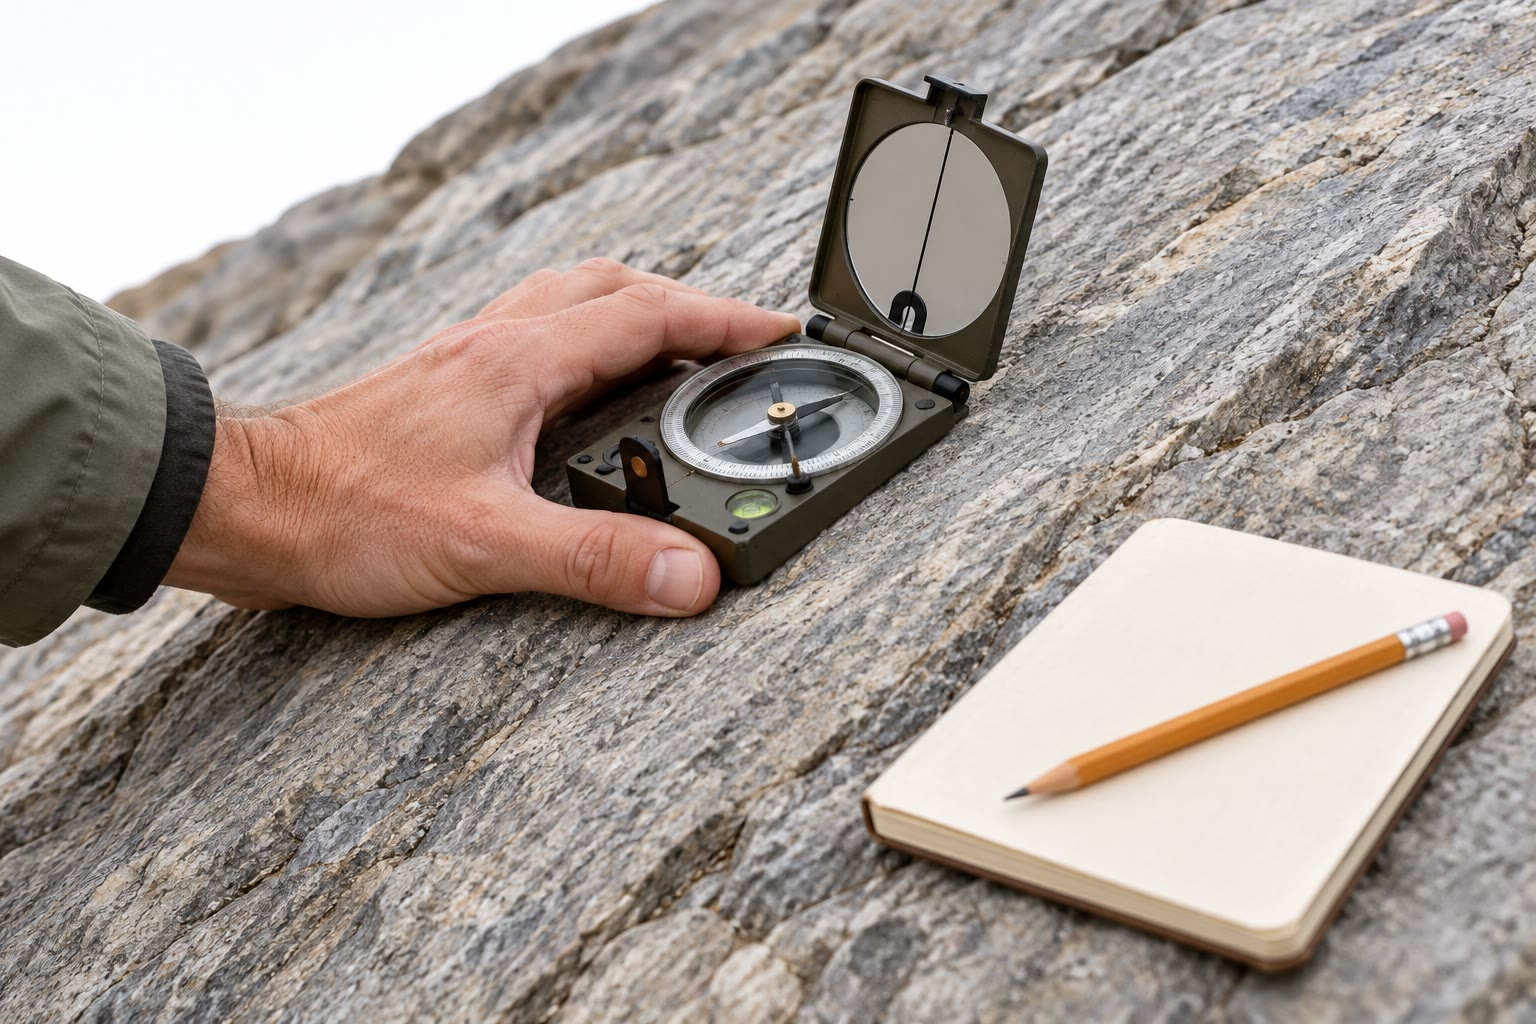
\includegraphics[width=\linewidth]{images/book5/ai/b3-compass-clinometer.jpg}

{\scriptsize झुकी चट्टान की सतह से सटाकर रखा गया एक कंपास-क्लाइनोमीटर, साथ में
एक क्षेत्र नोटबुक (AI से बनाया गया चित्रण)।}
\end{minipage}
\end{inthefield}

\section{अभ्यास}

\begin{exercise}[$\star$]\label{exo:b3:structural-analysis:1}
समतल $040/30$ के \omterm{def:b3:structural-analysis:stereo}{ध्रुव} का दिगंश और नमन ज्ञात कीजिए (नति-दिशा,
नति)। वह समतल ज्ञात कीजिए जिसके \omterm{def:b3:structural-analysis:stereo}{ध्रुव} का दिगंश \ang{315}
और नमन \ang{20} है।
\end{exercise}

\begin{exercise}[$\star$]\label{exo:b3:structural-analysis:2}
एक रेखा का नमन \ang{30} है। केंद्र से किस दूरी पर वह \omterm{def:b3:structural-analysis:stereo}{सम-कोणीय जाल} पर
और सम-क्षेत्रफल जाल पर अंकित होती है, जब दोनों जालों की त्रिज्या \qty{10}{cm} हो?
\end{exercise}

\begin{exercise}[$\star$]\label{exo:b3:structural-analysis:3}
किसी वलन के पार्श्वों के अभिविन्यास $090/30$ और $270/30$ हैं। इनके ध्रुवों के बीच का
कोण अभिलंबों के डॉट गुणनफल से, अंतर-पार्श्व कोण
और वलन का वर्ग परिकलित कीजिए।
\end{exercise}

\begin{exercise}[$\star$]\label{exo:b3:structural-analysis:4}
एक भ्रंश $090/60$ पर \ang{-45} रेक की धारियाँ हैं। स्ट्राइक सदिश
$\vec s = (0, 1, 0)$ और समतल के नीचे-नति सदिश $\vec d$ लेकर, ऊपरी भित्ति का सर्पण
$\vec u = \cos r\,\vec s - \sin r\,\vec d$ है। नीचे की राशियाँ
$\vec d$, $\vec u$ और सर्पण का दिगंश तथा नमन परिकलित कीजिए। भ्रंश का नाम दीजिए।
\end{exercise}

\begin{exercise}[$\star\star$]\label{exo:b3:structural-analysis:5}
किसी वलन के पार्श्वों के अभिविन्यास $060/40$ और $250/30$ हैं। इसके वलन-अक्ष का
दिगंश और नमन, तथा अंतर-पार्श्व कोण परिकलित कीजिए।
\end{exercise}

\begin{exercise}[$\star\star$]\label{exo:b3:structural-analysis:6}
वृत्त के भीतर पड़ने वाले जाल के क्षेत्रफल का वह भाग,
जिसमें \ang{60} से अधिक नमन वाली रेखाएँ हैं, सम-क्षेत्रफल और \omterm{def:b3:structural-analysis:stereo}{सम-कोणीय जाल} पर,
और निचले गोलार्ध की उन दिशाओं का भाग जिनका नमन
\ang{60} से अधिक है, परिकलित कीजिए। ध्रुवों की गिनती के लिए किस जाल का उपयोग करना चाहिए?
\end{exercise}

\begin{exercise}[$\star\star$]\label{exo:b3:structural-analysis:7}
तीन \omterm{def:b3:structural-analysis:stereo}{ध्रुव} ऊर्ध्वाधर पूर्व--पश्चिम तल में पड़ते हैं, ऊर्ध्वाधर से \ang{-20}, $0$ और
\ang{20} दूर: $\vec p = (\sin a, 0, -\cos a)$। इनका
\omterm{def:b3:structural-analysis:orientation-tensor}{अभिविन्यास प्रदिश}, उसके आइगेनमान और आइगेनसदिश, तथा \omterm{def:b3:structural-analysis:pi}{बीटा-अक्ष} परिकलित कीजिए। क्यों
सबसे छोटा आइगेनमान ठीक शून्य है?
\end{exercise}

\begin{exercise}[$\star\star$]\label{exo:b3:structural-analysis:8}
फ़्लिन आरेख पर दीर्घवृत्तज $X : Y : Z = 3 : 1.5 : 1$ अंकित कीजिए, फिर
स्थिर आयतन वाला दीर्घवृत्तज, जिसमें $X = 1.8$ और $Y = 1.1$ है। प्रत्येक के लिए $k$ परिकलित कीजिए
और विकृति का नाम दीजिए।
\end{exercise}

\begin{exercise}[$\star\star$]\label{exo:b3:structural-analysis:9}
स्ट्रेच के समांतर काटे गए एक काट में, आरंभ में गोल ऊइड
सभी समांतर, अक्षीय अनुपात $2.25$ वाले दीर्घवृत्त हैं, और प्रत्येक का क्षेत्रफल
अपरिवर्तित है। मुख्य स्ट्रेच और लंबे
अक्ष के अनुदिश प्रसार परिकलित कीजिए। विकृति से पहले ऊइड के केंद्र कभी
\qty{0.4}{mm} से निकट नहीं थे: \omterm{def:b3:structural-analysis:strain-analysis}{फ़्राई विधि} के आलेख के रिक्त क्षेत्र के अर्ध-अक्ष दीजिए।
\end{exercise}

\begin{exercise}[$\star\star\star$]\label{exo:b3:structural-analysis:10}
नादिर से $\theta = \ang{60}$ पर, त्रिज्या के अनुदिश स्ट्रेच
$\mathrm dr/(R\,\mathrm d\theta)$, और वृत्त के चारों ओर $r/(R\sin\theta)$,
दोनों प्रक्षेपणों के लिए परिकलित कीजिए। प्रक्षेपणों पर प्रमेय की जाँच कीजिए, और जिस अंडाकार में
\omterm{def:b3:structural-analysis:stereo}{सम-क्षेत्रफल प्रक्षेपण} वहाँ एक अति छोटे वृत्त को बदल देता है, उसके अक्षों का
अनुपात दीजिए।
\end{exercise}

\begin{exercise}[$\star\star\star$]\label{exo:b3:structural-analysis:11}
स्ट्राइक-स्लिप शासन में, $\sigma_1$ \ang{000} की ओर क्षैतिज है,
$\sigma_3$ \ang{090} की ओर क्षैतिज और $\sigma_2$ ऊर्ध्वाधर है। एक ऊर्ध्वाधर
भ्रंश का स्ट्राइक \ang{020} है। $\vec\tau$ परिकलित किए बिना दिखाइए कि इसका सर्पण
हर $\Phi$ के लिए क्षैतिज है। $-\vec\tau$ परिकलित कीजिए, $\Phi = 0.4$ लेकर,
समतल के अभिलंब $\vec n = (\cos\ang{20}, -\sin\ang{20}, 0)$ के साथ, और
सर्पण की दिशा बताइए।
\end{exercise}

\begin{exercise}[$\star\star\star$]\label{exo:b3:structural-analysis:12}
\qty{20}{km} लंबी एक काट विलगन वलनों की श्रेणी को पार करती है। दो क्षितिज
\qty{1.0}{km} दूर हैं और अपने मूल स्तर से ऊपर उठे हैं, जिनके क्षेत्रफल
\qty{6.0}{km^2} (निचला) और \qty{7.5}{km^2} (ऊपरी) हैं। लघुकरण,
निचले क्षितिज से नीचे विलगन की गहराई, काट की मूल लंबाई
और उसकी लंबाई का सापेक्षिक परिवर्तन परिकलित कीजिए।
\end{exercise}

\section{समस्या: वार्डन पहाड़ियों के वलन और भ्रंश}

\begin{problem}[{सप्ताहांत समस्या --- एक वलन का अक्ष, एक भ्रंश-समूह का प्रतिबल
और एक काट का पुनर्स्थापन, एक काल्पनिक क्षेत्र में}]
\label{pb:b3:structural-analysis:1}
% values: calc/ch08.py; figdata/bachelor-3/stereonet.py (data invented from region.py)
वार्डन पहाड़ियों में, जो श्रेणी का काल्पनिक क्षेत्र है, एक मेसोज़ोइक आवरण
शिस्ट और ग्रेनाइट के आधार पर टिका है। आवरण सीधे पार्श्वों वाली एक अपनति
और अभिनति में वलित है, फिर उसे एक सामान्य भ्रंश काटता है।
एक भूवैज्ञानिक ने अपनति के दोनों पार्श्वों पर बारह संस्तर-तल मापे
(नति-दिशा/नति, अंशों में):

\begin{center}
\small
\begin{tabular}{l|cccccc}
\hline
पूर्वी पार्श्व & 075/13 & 084/11 & 089/13 & 079/14 & 086/12 & 072/11 \\
पश्चिमी पार्श्व & 283/11 & 272/13 & 281/14 & 288/10 & 276/13 & 274/12 \\
\hline
\end{tabular}
\end{center}

प्रत्येक पार्श्व के छह मापनों के ऊर्ध्वगामी इकाई-अभिलंबों के योग
$\vec S_E = (1.2583, 0.2017, 5.8604)$ और $\vec S_W = (-1.2445, 0.1886,
5.8636)$ हैं (पूर्व, उत्तर, ऊपर)। पाँच भ्रंशों पर सर्पण-रेखाएँ अंकित हैं
(नति-दिशा/नति, ऊपरी भित्ति के सर्पण का रेक): $120/60/{-90}$ (मुख्य भ्रंश), $150/55/{-76}$,
$090/65/{-108}$, $200/70/{-78}$ और $060/50/{-105}$। मुख्य भ्रंश का
विस्थापन \qty{200}{m} है। अपनति और अभिनति के अक्ष \qty{4}{km} दूर हैं,
इसलिए वलन पूर्व से पश्चिम की ओर \qty{8}{km} पर दोहराते हैं।

\medskip\noindent\textbf{भाग I --- ध्रुव और बीटा-अक्ष।}
\begin{enumerate}
  \item मापन $075/13$ के \omterm{def:b3:structural-analysis:stereo}{ध्रुव} की दिगंश और नमन, और
        सम-क्षेत्रफल जाल के केंद्र से उसकी दूरी, जिसकी त्रिज्या
        \qty{10}{cm} है, भी दीजिए।
  \item मापन $075/13$ का ऊर्ध्वगामी इकाई-अभिलंब परिकलित कीजिए; उसे
        परिमाण में $\vec S_E$ के साथ जाँचिए।
  \item $\vec S_E$ और $\vec S_W$ से प्रत्येक पार्श्व का माध्य अभिविन्यास,
        माध्य परिणामी लंबाइयाँ, और मापनों का
        उनके माध्य के सापेक्ष वर्ग-माध्य-मूल प्रकीर्णन परिकलित कीजिए।
  \item $\vec S_E\times\vec S_W$ तथा \omterm{def:b3:structural-analysis:pi}{बीटा-अक्ष} की दिगंश और नमन
        परिकलित कीजिए।
  \item दोनों माध्य अभिलंबों के बीच का कोण, अंतर-पार्श्व कोण
        और वलन का वर्ग परिकलित कीजिए।
  \item इस सममित वलन का अक्षीय तल \omterm{def:b3:structural-analysis:pi}{बीटा-अक्ष} को समाविष्ट करता है और
        $\vec m_E - \vec m_W$ पर लंब होता है, जो माध्य इकाई-अभिलंबों का अंतर है।
        इसका अभिविन्यास दीजिए; क्या वलन सीधा है?
  \item $\pi$-पट्टी का अभिविन्यास दीजिए, और बताइए कि \omterm{def:b3:structural-analysis:stereo}{ध्रुव} उस पर
        क्यों स्थित हैं।
\end{enumerate}

\medskip\noindent\textbf{भाग II --- अभिविन्यास प्रदिश।}
बारह ध्रुवों का \omterm{def:b3:structural-analysis:orientation-tensor}{अभिविन्यास प्रदिश}
\[
  T = \begin{pmatrix} 0.04400 & 0.00035 & 0.00109\\ 0.00035 & 0.00144 & 0.03179\\
  0.00109 & 0.03179 & 0.95456 \end{pmatrix},
\]
जिसके आइगेनमान $0.95562$, $0.04400$ और $0.00038$ हैं।
\begin{enumerate}[resume]
  \item जाँचिए कि $T$ का अनुरेख 1 है। $\vec b = (0.0053, -0.9994,
        0.0333)$ लेकर, जो $\vec S_E\times\vec S_W$ की दिशा का इकाई सदिश है,
        $\vec b^{\mathsf T}T\vec b$ परिकलित कीजिए। यह परिणाम $\vec b$ के बारे में क्या कहता है?
  \item ध्रुवों और पट्टी के बीच का वर्ग-माध्य-मूल कोण परिकलित कीजिए।
  \item पार्श्वों की नतियों से $\lambda_2$ का मान समझाइए।
  \item मापनों की परिशुद्धता के भीतर क्या वलन बेलनाकार है?
  \item \omterm{def:b3:structural-analysis:pi}{बीटा-अक्ष} का नमन पट्टी के उत्तर--दक्षिण झुकाव से निर्धारित होता है,
        पट्टी, जिसमें हर \omterm{def:b3:structural-analysis:stereo}{ध्रुव} अपना योगदान
        प्रश्न 9 में मिले प्रकीर्णन के साथ देता है। नमन की मानक त्रुटि आकलित कीजिए।
\end{enumerate}

\medskip\noindent\textbf{भाग III --- पुरा-प्रतिबल।}
\begin{enumerate}[resume]
  \item मुख्य भ्रंश किस प्रकार का है? एंडरसन के अनुसार
        $\sigma_1$, $\sigma_2$ और $\sigma_3$ की दिशाएँ दीजिए।
  \item सर्पण-दिशा के प्रमेय से दिखाइए कि मुख्य भ्रंश सीधे अपनी नति के
        अनुदिश नीचे सरकता है, चाहे $\Phi$ का मान कुछ भी हो।
        यह $\Phi$ के बारे में क्या बताता है?
  \item भ्रंश $150/55$ के लिए $\vec n$ तथा उसके घटक $n_1 =
        \vec n\cdot\vec e_1$ और $n_2 = \vec n\cdot\vec e_2$ परिकलित कीजिए, $\vec e_1$ को
        ऊर्ध्वाधर और $\vec e_2$ को \ang{030} की ओर क्षैतिज मानकर।
  \item इसका सर्पण $\vec w = \vec n\times\vec u = (0.771, 0.605, 0.198)$ देता है।
        $\Phi$ परिकलित कीजिए।
  \item अन्य तीन छोटे भ्रंश $\Phi = 0.294$, $0.301$ और
        $0.306$ के मान देते हैं। माध्य दीजिए, और बताइए कि प्रसार कहाँ से आता है।
  \item $\Phi = 0.3$ $\sigma_2$ के बारे में क्या कहता है?
  \item मुख्य भ्रंश के P और T अक्ष (तल से \ang{45} पर, उसके
        नति-तल में) परिकलित कीजिए, और उनकी $\sigma_1$ और
        $\sigma_3$ से तुलना कीजिए।
\end{enumerate}

\medskip\noindent\textbf{भाग IV --- पूर्व--पश्चिम काट का पुनर्स्थापन।}
\begin{enumerate}[resume]
  \item पूर्वी पार्श्व की आभासी नति, $080.9/12.3$, पूर्व--पश्चिम काट पर
        परिकलित कीजिए।
  \item काट पर पार्श्वों को \ang{12} पर लेकर, एक वलन-तरंगदैर्घ्य की पुनर्स्थापित
        लंबाई, लघुकरण और लंबाई का सापेक्षिक परिवर्तन
        परिकलित कीजिए।
  \item अभिनतियों से ऊपर अपनति-शिखर की ऊँचाई और
        एक तरंगदैर्घ्य का अतिरिक्त क्षेत्रफल परिकलित कीजिए, यह मानकर कि अभिनतियाँ
        मूल स्तर पर बनी रहीं।
  \item वलित संस्तर के नीचे विलगन की गहराई परिकलित कीजिए। क्या वलन
        आवरण के आधार पर, कुछ सौ मीटर
        नीचे, विलगित हो सकते हैं?
  \item \ang{120} की दिशा वाली काट पर मुख्य भ्रंश का क्षैतिज विस्थापन
        और सर्पण परिकलित कीजिए।
  \item पूर्व--पश्चिम काट पर भ्रंश की आभासी नति और उसका
        आभासी क्षैतिज विस्थापन परिकलित कीजिए। किस काट का पुनर्स्थापन करना चाहिए?
  \item भ्रंश और वलनों का पुनर्स्थापन किस क्रम में होता है, और \omterm{def:b3:structural-analysis:restoration}{पिन रेखाएँ}
        कहाँ रखी जाती हैं?
  \item बारह मापनों से पुनःप्राप्त वार्डन वलन-अक्ष का नमन
        क्या है?
\end{enumerate}
\end{problem}
